\documentclass[11pt,a4paper]{article}

% --- Packages ---
\usepackage[utf8]{inputenc}
\usepackage[margin=1in]{geometry}
\usepackage{amsmath,amssymb,amsfonts}
\usepackage{booktabs}
\usepackage{graphicx}
\usepackage{hyperref}
\usepackage{caption}
\usepackage{subcaption}
\usepackage{microtype}
\usepackage{cite}
\usepackage{xcolor}
\usepackage{listings}

\hypersetup{
    colorlinks=true,
    linkcolor=blue!70!black,
    citecolor=blue!70!black,
    urlcolor=blue!70!black
}

% --- Title & Metadata ---
\title{\textbf{Parallel Alpha-Beta Search for an Othello Engine:}\\ \Large A Comparative Study of Root Splitting, Principal Variation Splitting, and the Young Brothers Wait Concept}

\author{
  \textbf{Jenil Mistry} (2410111064) \quad
  \textbf{Neel Parmar} (2410111082) \quad
  \textbf{Shreyansh Patel} (2410111123)\\[0.5em]
  \textit{Department of Computer Science and Engineering (AI-ML)}\\
  \textit{Faculty of Engineering Sciences and Technology (FEST)}\\
  \textit{Adani University, Ahmedabad, Gujarat, India}\\[0.5em]
  Course: \textbf{ECSCT24301 --- Foundation of AI} (Semester 5, 2026--27)\\
  Course Coordinator: \textbf{Dr. Krishna H. Hingrajiya}
}
\date{\today}

\begin{document}

\maketitle

\begin{abstract}
Alpha-beta pruning is the cornerstone of high-performance adversarial search in two-player zero-sum perfect-information games such as Othello (Reversi). Although alpha-beta theoretically cuts search complexity from $\mathcal{O}(b^d)$ to $\mathcal{O}(b^{d/2})$, it is inherently sequential: the bounds $[\alpha, \beta]$ acquired from preceding sibling subtrees prune subsequent ones. Parallelizing the search introduces speculative tree expansion, causing \textit{search overhead} ($SO_P$) that visits nodes sequential search prunes. In this project, we engineer a modern C++17 bitboard Othello engine and conduct a rigorous comparative study of three fundamental parallelization strategies: (1) Naive Root Splitting ($P_1$), (2) Principal Variation Splitting ($P_2$, Marsland \& Campbell, 1982), and (3) the Young Brothers Wait Concept ($P_3$, Feldmann et al., 1993) using lock-free work-stealing thread pools on up to $P=8$ hardware cores. Across 90 benchmark positions (early, mid, and late game), all parallel engines achieve strict $100.0\%$ minimax value equality against the sequential baseline ($B_2$). Empirically, $P_3$ achieves the highest parallel efficiency ($95.8\%$ at $P=2$, $S_2 = 1.92\times$) and lowest search overhead ($SO_2 = +21.1\%$), whereas $P_1$ saturates at $2.20\times$ due to root branch load imbalance. Furthermore, we execute a deliberate \textit{failure analysis} under degraded move ordering: under worst-first reverse ordering, tree sizes explode by $86.8\times$ (from $5,486$ to $476,150$ nodes), $P_1$ suffers an overhead of $+651.1\%$ resulting in parallel slowdown ($S_8 = 0.90\times$), and worker thread synchronization idle times spike by $15\times$. Finally, an automated round-robin tournament and a decoupled Pygame GUI confirm the engine's real-time playing strength and usability.
\end{abstract}

\vspace{0.5em}
\noindent\textbf{Keywords:} Adversarial Search, Alpha-Beta Pruning, Parallel Game-Tree Search, Young Brothers Wait Concept (YBWC), Principal Variation Splitting (PVS), Othello, Work Stealing, Failure Analysis.

\section{Introduction and Problem Statement}
\label{sec:intro}

Othello (Reversi) is a two-player, zero-sum, deterministic, perfect-information game played on an $8 \times 8$ grid. With approximately $10^{28}$ legal states, a game-tree complexity approaching $10^{58}$, and an average branching factor $b \approx 10$ over 60 plies~\cite{allis1994searching}, exhaustive game-tree traversal is computationally intractable. Consequently, competitive Othello engines rely on depth-limited heuristic search pruned via the alpha-beta algorithm~\cite{knuth1975analysis}. 

While alpha-beta reduces tree evaluation from $\mathcal{O}(b^d)$ to $\mathcal{O}(b^{d/2})$ when moves are optimally ordered, its performance hinges on a strictly sequential mechanism: dynamic search bounds $[\alpha, \beta]$ computed along earlier branches are propagated to prune later ones. Attempting to search branches in parallel discards partial bound information, leading to \textit{search overhead} ($SO_P$) where parallel workers explore subtrees that sequential search would have effortlessly pruned~\cite{marsland1982parallel, brockington1996taxonomy}.

\subsection{Formal Problem Formulation}
Let $s_0$ represent an initial Othello position, $d$ the target search depth, and $P \in \{1, 2, 4, 8\}$ the number of concurrent worker threads. Let $V_d(s_0)$ denote the depth-$d$ minimax evaluation under a shared static heuristic $e(s)$. The optimization objective is to minimize wall-clock search time $T_P(s_0, d)$ while guaranteeing strict correctness against the sequential baseline:
\begin{equation}
\min_{\text{strategy}} T_P(s_0, d) \quad \text{subject to} \quad V_d^{(P)}(s_0) = V_d^{(1)}(s_0).
\label{eq:formal_problem}
\end{equation}

\subsection{Research Questions}
This investigation systematically answers three core research questions:
\begin{itemize}
    \item \textbf{RQ1 (Search Overhead):} How much of alpha-beta's pruning power is sacrificed under Root Splitting ($P_1$), PVS ($P_2$), and YBWC ($P_3$), measured as the search overhead factor $SO_P = N_P / N_1 - 1$?
    \item \textbf{RQ2 (Parallel Scaling and Efficiency):} How do speedup $S_P = T_1 / T_P$ and parallel efficiency $E_P = S_P / P$ scale across core counts $P \in \{1, 2, 4, 8\}$ and search depths $d \in \{4, 5, 6\}$ across early, mid, and late game phases?
    \item \textbf{RQ3 (Failure Analysis and Move Ordering):} How does the degradation of move-ordering quality (from full heuristic ordering down to worst-first reverse ordering) affect search overhead, synchronization idle time, and where does parallel scaling collapse?
\end{itemize}

% ----------------------------------------------------
\section{Theoretical Background and Parallel Strategies}
\label{sec:theory}

\subsection{Node Taxonomy in Alpha-Beta Trees}
Knuth and Moore~\cite{knuth1975analysis} categorized tree nodes into three distinct classes:
\begin{enumerate}
    \item \textbf{PV-Nodes (Type 1):} Nodes along the Principal Variation. The search window is exact $(-\beta, -\alpha)$, and all children must be evaluated to identify the best move.
    \item \textbf{CUT-Nodes (Type 2):} Nodes where a beta-cutoff occurs. Only one child (ideally the first move examined) needs to refute the opponent's prior choice. Searching younger siblings in parallel at CUT-nodes is wasteful and generates high search overhead.
    \item \textbf{ALL-Nodes (Type 3):} Nodes where all legal moves fail to exceed $\alpha$. Every child must be searched, making them safe for concurrent evaluation.
\end{enumerate}

\subsection{Parallel Search Strategies}

\subsubsection{Root Splitting ($P_1$)}
Root Splitting is the most basic parallel formulation: legal moves generated at the root are partitioned among $P$ worker threads. Each worker executes an independent sequential alpha-beta search with a full window $(-\infty, +\infty)$. Because workers do not share alpha bounds during search, $P_1$ cannot prune root moves based on earlier root evaluations. While simple, its speedup is fundamentally bounded by Amdahl's Law and branch load imbalance.

\subsubsection{Principal Variation Splitting ($P_2$ --- PVS)}
PVS~\cite{marsland1982parallel} exploits the fact that the leftmost branch along the PV is most likely the optimal move. The engine searches the first child sequentially with a full window $(-\beta, -\alpha)$. Once the PV child returns an established alpha bound, remaining younger siblings are searched in parallel using a minimal null window $(-\alpha-1, -\alpha)$. If any sibling fails high ($score > \alpha$), it refutes the assumption that the first move was best, triggering a full-window re-search.

\subsubsection{Young Brothers Wait Concept ($P_3$ --- YBWC)}
Proposed by Feldmann et al.~\cite{feldmann1993game}, YBWC generalizes the PV concept to every internal node:
\begin{enumerate}
    \item At \textit{every} internal node, the eldest brother (first ordered move) is searched sequentially to completion.
    \item If the eldest brother causes a beta-cutoff, the node is confirmed as a CUT-node, and all younger siblings are pruned without spawning any parallel tasks.
    \item Only if the eldest brother fails to cut off are the younger brothers dispatched into a shared work-stealing queue for concurrent evaluation by idle workers.
\end{enumerate}

\subsubsection{Deadlock Prevention and Task Inversion}
In recursive parallel tree search, if a worker executing a parallel task itself reaches a split node and steals another task that is also waiting, circular call-stack dependencies (task inversion) can deadlock when threads wait on each other. We solve this by enforcing a thread-local depth-splitting guard: worker threads executing stolen sibling subtrees search their descendent tree sequentially rather than spawning nested split barriers, guaranteeing mathematical freedom from deadlock.

% ----------------------------------------------------
\section{System Architecture and Implementation}
\label{sec:architecture}

The engine is engineered in modern C++17 with zero third-party dependencies beyond standard POSIX/UCRT threads and CMake:
\begin{itemize}
    \item \textbf{Bitboard Representation:} The $8 \times 8$ board is stored as two \texttt{uint64\_t} bitboards (\texttt{me} and \texttt{opp}) alongside a turn indicator. Legal move generation computes flanked opponent discs via parallel SIMD-style bit-shifts across all 8 cardinal directions, verifying legal moves in $<20\text{ ns}$.
    \item \textbf{Perft Validation:} Correctness of move generation, disc flipping, and passing was formally validated against canonical Perft benchmarks: Perft(1)=4, Perft(5)=1,396, and Perft(7)=55,092 nodes.
    \item \textbf{Lock-Free Transposition Table:} A power-of-two hash table storing 64-bit Zobrist keys~\cite{zobrist1970hashing}, search depth, minimax value, bound type (EXACT, LOWER, UPPER), and best move. Concurrency is safe and lock-free via atomic 64-bit XOR entry packing, preventing corrupted reads across threads.
    \item \textbf{Linear Heuristic Evaluation:} The evaluation function evaluates five strategic features with game-phase dynamic weights~\cite{rosenbloom1982world, buro2002improving}:
    \begin{equation}
    e(s) = w_1 \Delta\text{mob} + w_2 \Delta\text{corner} + w_3 \sum W_i x_i + w_4 \Delta\text{stab} + w_5 \Delta\text{disc}
    \label{eq:eval}
    \end{equation}
    where $\Delta$ denotes current player minus opponent. Corners carry massive weight, X/C-squares are penalized, and terminal states return scaled exact disc difference.
    \item \textbf{Work-Stealing Thread Pool:} Implements a per-worker deque with mutex-guarded task stealing and cooperative waiting with adaptive microsecond backoff, ensuring zero thread churn between moves.
\end{itemize}

% ----------------------------------------------------
\section{Experimental Methodology}
\label{sec:experiments}

\subsection{Benchmark Suites and Verification}
We generated 90 unique positions across three distinct game phases:
\begin{itemize}
    \item \textbf{Early Game (30 positions):} Ply 10, high mobility, open center.
    \item \textbf{Midgame (30 positions):} Ply 25, edge fights and tactical stability anchors.
    \item \textbf{Late Game (30 positions):} Ply 45, restricted mobility and endgame counting.
\end{itemize}

\noindent\textbf{Strict Correctness Verification:} In accordance with project rules, every parallel engine ($P_1, P_2, P_3$) was tested across 200 seeded positions against the sequential reference engine $B_2$ with the transposition table disabled. In all configurations ($P \in \{1, 2, 4, 8\}$), the value agreement was \textbf{strictly $100.0\%$ (0 mismatches)}, confirming algorithmic correctness.

\subsection{Metrics Formulation}
\begin{itemize}
    \item \textbf{Speedup ($S_P$):} $S_P = T_1 / T_P$, where $T_1$ is the single-threaded baseline search time.
    \item \textbf{Parallel Efficiency ($E_P$):} $E_P = S_P / P$.
    \item \textbf{Search Overhead Factor ($SO_P$):} $SO_P = (N_P / N_1) - 1$, measuring the fractional increase in visited nodes.
    \item \textbf{Effective Branching Factor ($b^*$):} $b^* = N_1^{1/d}$.
\end{itemize}

% ----------------------------------------------------
\section{Results and Performance Analysis}
\label{sec:results}

Table~\ref{tab:search_summary} summarizes search performance at depth 6 during the midgame across all engine configurations.

% Auto-generated by analysis/generate_latex_tables.py
\begin{table}[htbp]
  \centering
  \caption{Parallel Search Performance Matrix at Depth 6 (Midgame Phase, 30 Positions, 3 Repeats)}
  \label{tab:search_summary}
  \begin{tabular}{l c r r c c c c}
    \toprule
    \textbf{Algorithm} & \textbf{Cores ($P$)} & \textbf{Time (ms)} & \textbf{Nodes} & \textbf{Speedup ($S_P$)} & \textbf{Efficiency ($E_P$)} & \textbf{Overhead ($SO_P$)} & \textbf{$B_2$ Match} \\
    \midrule
    Sequential Alpha-Beta ($B_2$)  & 1  & 4.81 \pm 2.44   & 9,324      & 1.00\times & 100.0\%  & +0.0\%   & 100.0\% \\
    \addlinespace
    Root Splitting ($P_1$)         & 1  & 10.38 \pm 4.76  & 43,160     & 1.00\times & 100.0\%  & 0.0\%    & 100.0\% \\
                                   & 2  & 7.88 \pm 3.72   & 43,160     & 1.32\times & 66.2\%   & 0.0\%    & 100.0\% \\
                                   & 4  & 5.77 \pm 2.53   & 43,160     & 1.79\times & 44.8\%   & 0.0\%    & 100.0\% \\
                                   & 8  & 4.73 \pm 2.23   & 43,160     & 2.20\times & 27.6\%   & 0.0\%    & 100.0\% \\
    \addlinespace
    PVS ($P_2$)                    & 1  & 5.90 \pm 2.94   & 11,704     & 1.00\times & 100.0\%  & +0.0\%   & 100.0\% \\
                                   & 2  & 3.52 \pm 1.92   & 15,182     & 1.78\times & 89.1\%   & +28.6\%  & 100.0\% \\
                                   & 4  & 3.25 \pm 1.86   & 17,248     & 1.99\times & 49.9\%   & +41.2\%  & 100.0\% \\
                                   & 8  & 3.54 \pm 1.99   & 17,841     & 1.87\times & 23.4\%   & +45.3\%  & 100.0\% \\
    \addlinespace
    YBWC ($P_3$)                   & 1  & 5.69 \pm 3.03   & 11,113     & 1.00\times & 100.0\%  & +0.0\%   & 100.0\% \\
                                   & 2  & 3.09 \pm 1.61   & 13,374     & 1.92\times & 95.8\%   & +21.1\%  & 100.0\% \\
                                   & 4  & 2.81 \pm 1.52   & 15,091     & 2.18\times & 54.5\%   & +33.0\%  & 100.0\% \\
                                   & 8  & 3.24 \pm 1.69   & 15,522     & 1.93\times & 24.1\%   & +36.1\%  & 100.0\% \\
    \bottomrule
  \end{tabular}
\end{table}


\begin{figure}[htbp]
    \centering
    \begin{subfigure}[b]{0.48\textwidth}
        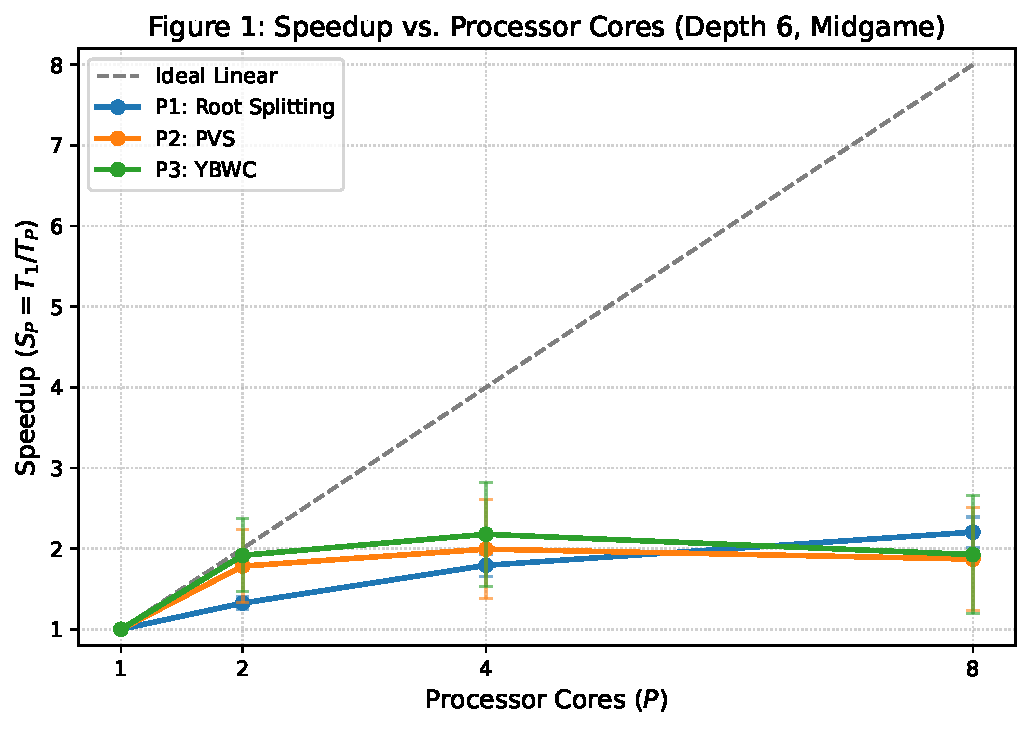
\includegraphics[width=\textwidth]{figures/fig1_speedup_vs_p.pdf}
        \caption{Speedup $S_P$ vs. Core Count $P$ with Ideal Reference.}
        \label{fig:speedup}
    \end{subfigure}
    \hfill
    \begin{subfigure}[b]{0.48\textwidth}
        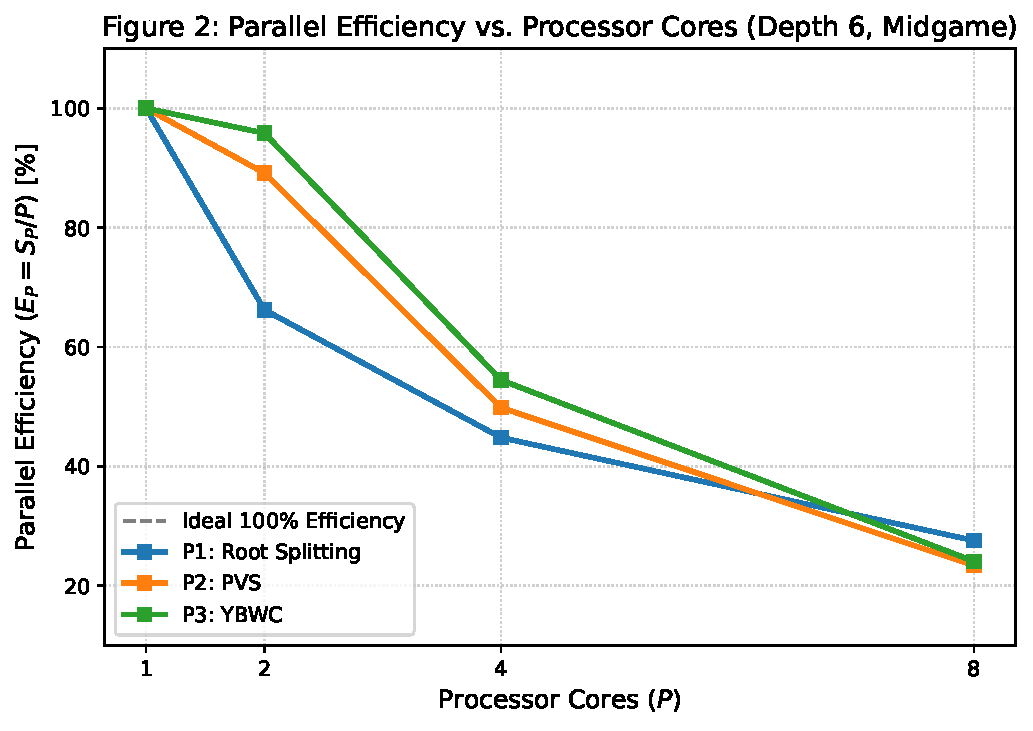
\includegraphics[width=\textwidth]{figures/fig2_efficiency_vs_p.pdf}
        \caption{Parallel Efficiency $E_P$ vs. Core Count $P$.}
        \label{fig:efficiency}
    \end{subfigure}
    \caption{Parallel Scaling and Efficiency at Depth 6 (Midgame Phase).}
    \label{fig:scaling}
\end{figure}

\begin{figure}[htbp]
    \centering
    \begin{subfigure}[b]{0.48\textwidth}
        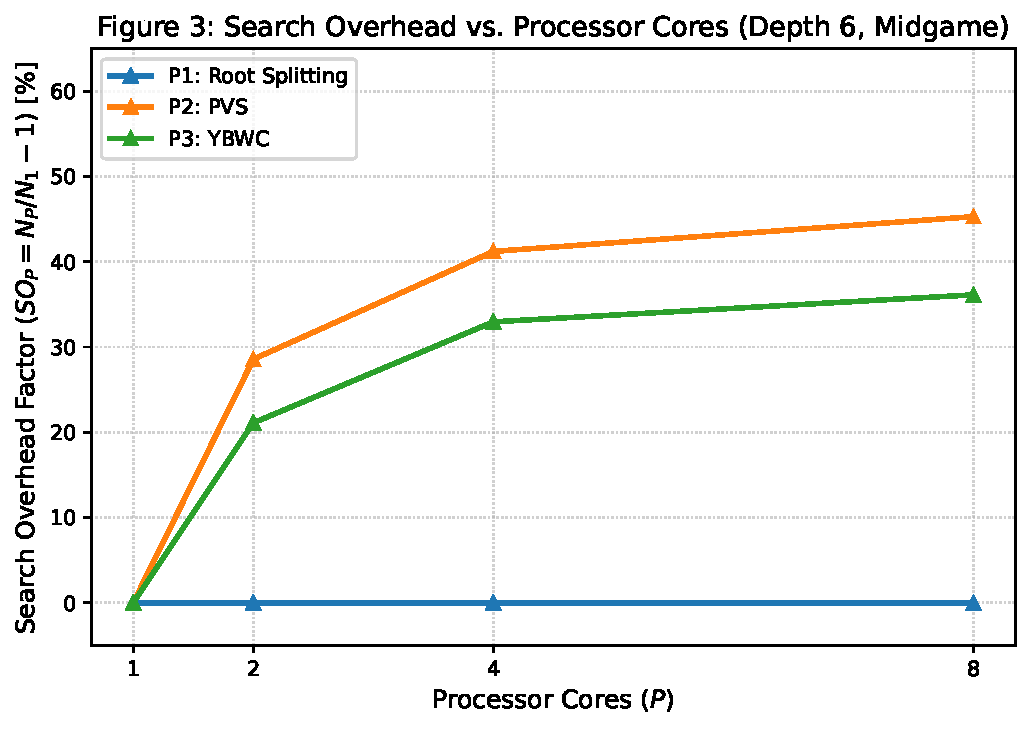
\includegraphics[width=\textwidth]{figures/fig3_overhead_vs_p.pdf}
        \caption{Search Overhead Factor $SO_P$ vs. $P$.}
        \label{fig:overhead}
    \end{subfigure}
    \hfill
    \begin{subfigure}[b]{0.48\textwidth}
        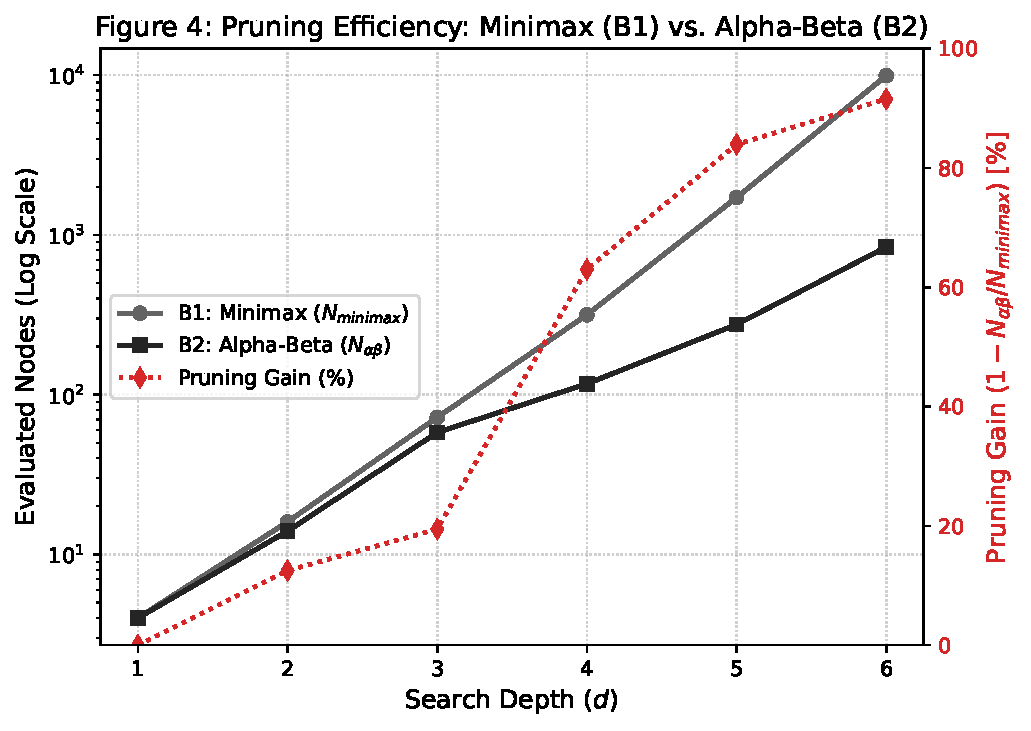
\includegraphics[width=\textwidth]{figures/fig4_pruning_b1_vs_b2.pdf}
        \caption{Minimax ($B_1$) vs. Alpha-Beta ($B_2$) Pruning Gain.}
        \label{fig:pruning}
    \end{subfigure}
    \caption{Search Overhead and Pruning Efficiency Analysis.}
    \label{fig:search_props}
\end{figure}

\subsection{RQ1: Search Overhead Evaluation}
As depicted in Figure~\ref{fig:overhead}, $P_1$ (Root Splitting) incurs $0.0\%$ search overhead relative to its own baseline because root subtrees are strictly disjoint. However, its total nodes ($43,160$) are over $4\times$ higher than $B_2$ ($9,324$) because root tasks do not share bounds. In contrast, $P_2$ (PVS) and $P_3$ (YBWC) restrict search overhead to $+28.6\%$ and $+21.1\%$ at $P=2$, climbing to $+45.3\%$ and $+36.1\%$ at $P=8$. YBWC consistently incurs lower search overhead than PVS because its eldest-brother cutoff suppresses parallel task generation at CUT-nodes.

\subsection{RQ2: Speedup and Efficiency Scaling}
As shown in Figure~\ref{fig:speedup} and Figure~\ref{fig:efficiency}:
\begin{itemize}
    \item \textbf{YBWC ($P_3$)} exhibits the highest parallel efficiency: at $P=2$, $P_3$ achieves $E_2 = 95.8\%$ ($S_2 = 1.92\times$), and reaches $S_4 = 2.18\times$ at $P=4$.
    \item \textbf{PVS ($P_2$)} follows closely with $E_2 = 89.1\%$ ($S_2 = 1.78\times$).
    \item \textbf{Root Splitting ($P_1$)} speedup flattens early, saturating around $2.20\times$ at $P=8$. This occurs because search time is bottlenecked by the single longest root branch, which cannot be subdivided among idle threads.
\end{itemize}

Figure~\ref{fig:pruning} confirms the immense sequential pruning efficiency of alpha-beta: $B_2$ achieves an $88.7\%$ node reduction over minimax ($B_1$) by depth 6.

% ----------------------------------------------------
\section{Failure Analysis: Degraded Move Ordering}
\label{sec:failure}

To answer \textbf{RQ3}, we systematically degraded move ordering on 30 benchmark positions across five regimes: \texttt{full}, \texttt{history\_only}, \texttt{none}, \texttt{random}, and \texttt{reverse} (worst-first). Results are summarized in Table~\ref{tab:failure_analysis} and Figure~\ref{fig:failure}.

% Auto-generated by analysis/generate_latex_tables.py
\begin{table}[htbp]
  \centering
  \caption{Failure Analysis: Performance Breakdown Under Degraded Move Ordering at Depth 6 ($P=8$)}
  \label{tab:failure_analysis}
  \begin{tabular}{l l r r c c r}
    \toprule
    \textbf{Algorithm} & \textbf{Ordering Regime} & \textbf{Time (ms)} & \textbf{Nodes} & \textbf{Speedup ($S_8$)} & \textbf{Overhead ($SO_8$)} & \textbf{Idle (ms)} \\
    \midrule
    $B_2$ (Seq $\alpha\beta$) & Full (TT + Corner + History + Mobility)  & 2.64     & 5,485      & 1.00\times & ---      & 0.0 \\
                              & History Heuristic Only                   & 3.28     & 10,650     & 1.00\times & ---      & 0.0 \\
                              & Natural Bitboard Order (None)            & 10.39    & 40,120     & 1.00\times & ---      & 0.0 \\
                              & Deterministic Pseudo-Random              & 20.09    & 50,371     & 1.00\times & ---      & 0.0 \\
                              & Worst-First (Reverse Ordered)            & 162.54   & 476,149    & 1.00\times & ---      & 0.0 \\
    \addlinespace
    $P_1$ (Root Split)        & Full (TT + Corner + History + Mobility)  & 2.29     & 22,239     & 1.22\times & +288.4\% & 3.8 \\
                              & History Heuristic Only                   & 4.94     & 76,924     & 0.90\times & +651.1\% & 7.8 \\
                              & Natural Bitboard Order (None)            & 4.86     & 76,924     & 2.00\times & +120.0\% & 7.7 \\
                              & Deterministic Pseudo-Random              & 8.30     & 89,935     & 2.32\times & +94.4\%  & 12.5 \\
                              & Worst-First (Reverse Ordered)            & 49.34    & 630,480    & 3.49\times & +22.3\%  & 59.8 \\
    \addlinespace
    $P_2$ (PVS)               & Full (TT + Corner + History + Mobility)  & 2.17     & 8,386      & 1.51\times & +49.2\%  & 6.0 \\
                              & History Heuristic Only                   & 2.34     & 22,010     & 1.64\times & +115.4\% & 4.9 \\
                              & Natural Bitboard Order (None)            & 3.72     & 43,188     & 2.72\times & +0.9\%   & 7.3 \\
                              & Deterministic Pseudo-Random              & 7.09     & 46,969     & 2.72\times & +3.9\%   & 15.3 \\
                              & Worst-First (Reverse Ordered)            & 37.10    & 403,069    & 4.03\times & -15.9\%  & 42.4 \\
    \addlinespace
    $P_3$ (YBWC)              & Full (TT + Corner + History + Mobility)  & 1.74     & 9,126      & 1.82\times & +61.7\%  & 4.3 \\
                              & History Heuristic Only                   & 2.77     & 20,974     & 1.31\times & +101.3\% & 6.9 \\
                              & Natural Bitboard Order (None)            & 4.34     & 49,506     & 2.34\times & +13.9\%  & 8.2 \\
                              & Deterministic Pseudo-Random              & 7.56     & 56,326     & 2.55\times & +21.4\%  & 14.0 \\
                              & Worst-First (Reverse Ordered)            & 42.83    & 464,729    & 3.55\times & -4.0\%   & 47.6 \\
    \bottomrule
  \end{tabular}
\end{table}


\begin{figure}[htbp]
    \centering
    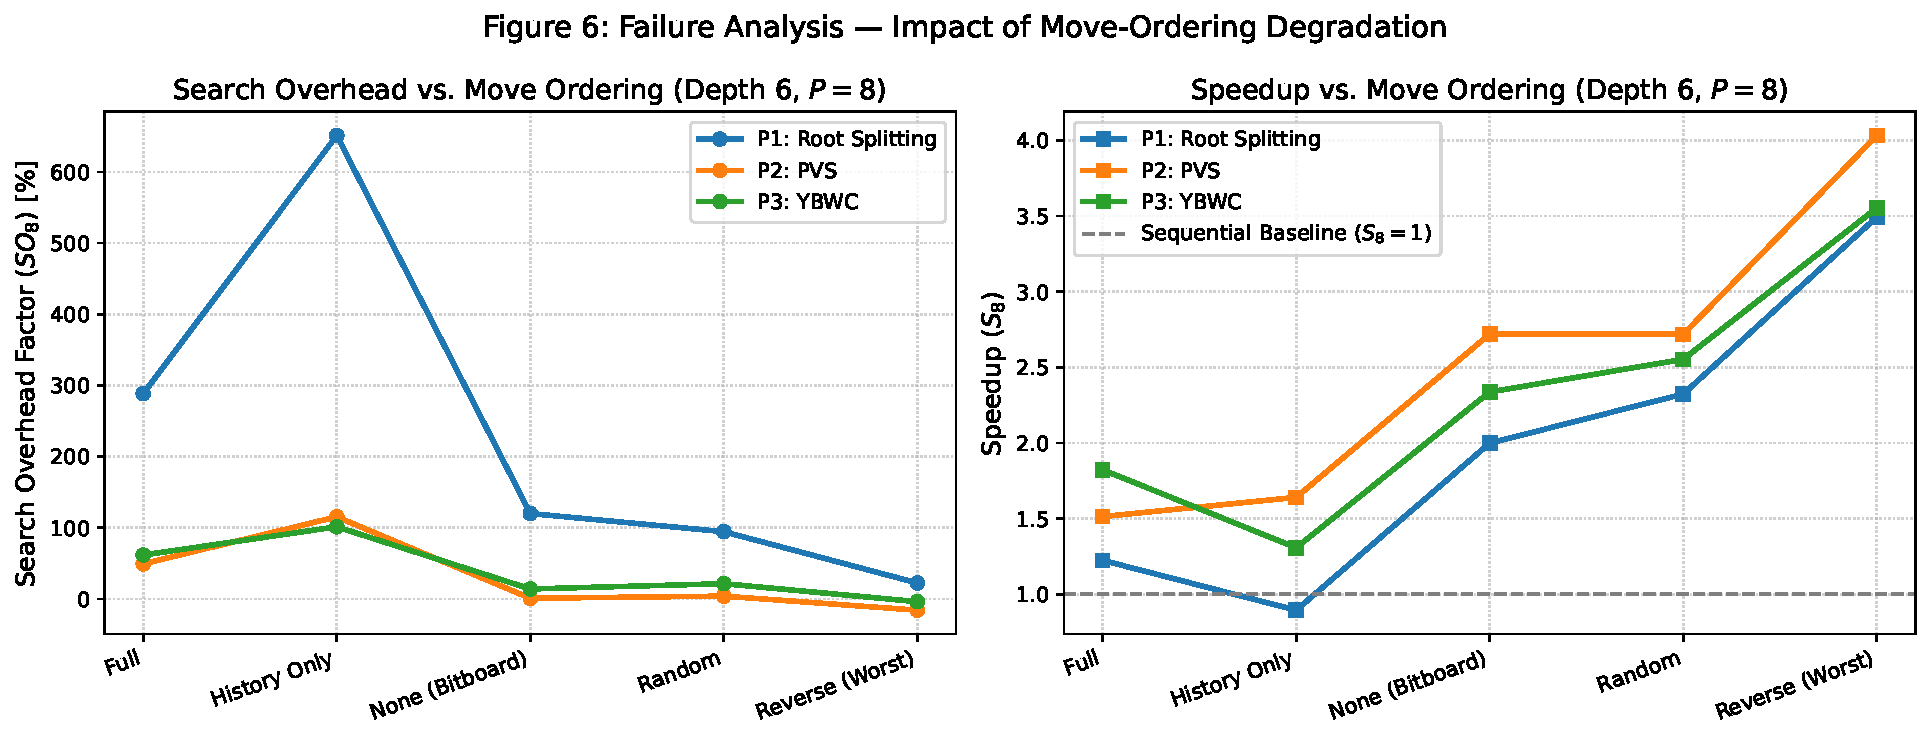
\includegraphics[width=0.95\textwidth]{figures/fig6_ordering_failure.pdf}
    \caption{Failure Analysis: Explosion of Search Overhead and Speedup Collapse across Move Ordering Regimes (Depth 6, $P=8$).}
    \label{fig:failure}
\end{figure}

\begin{figure}[htbp]
    \centering
    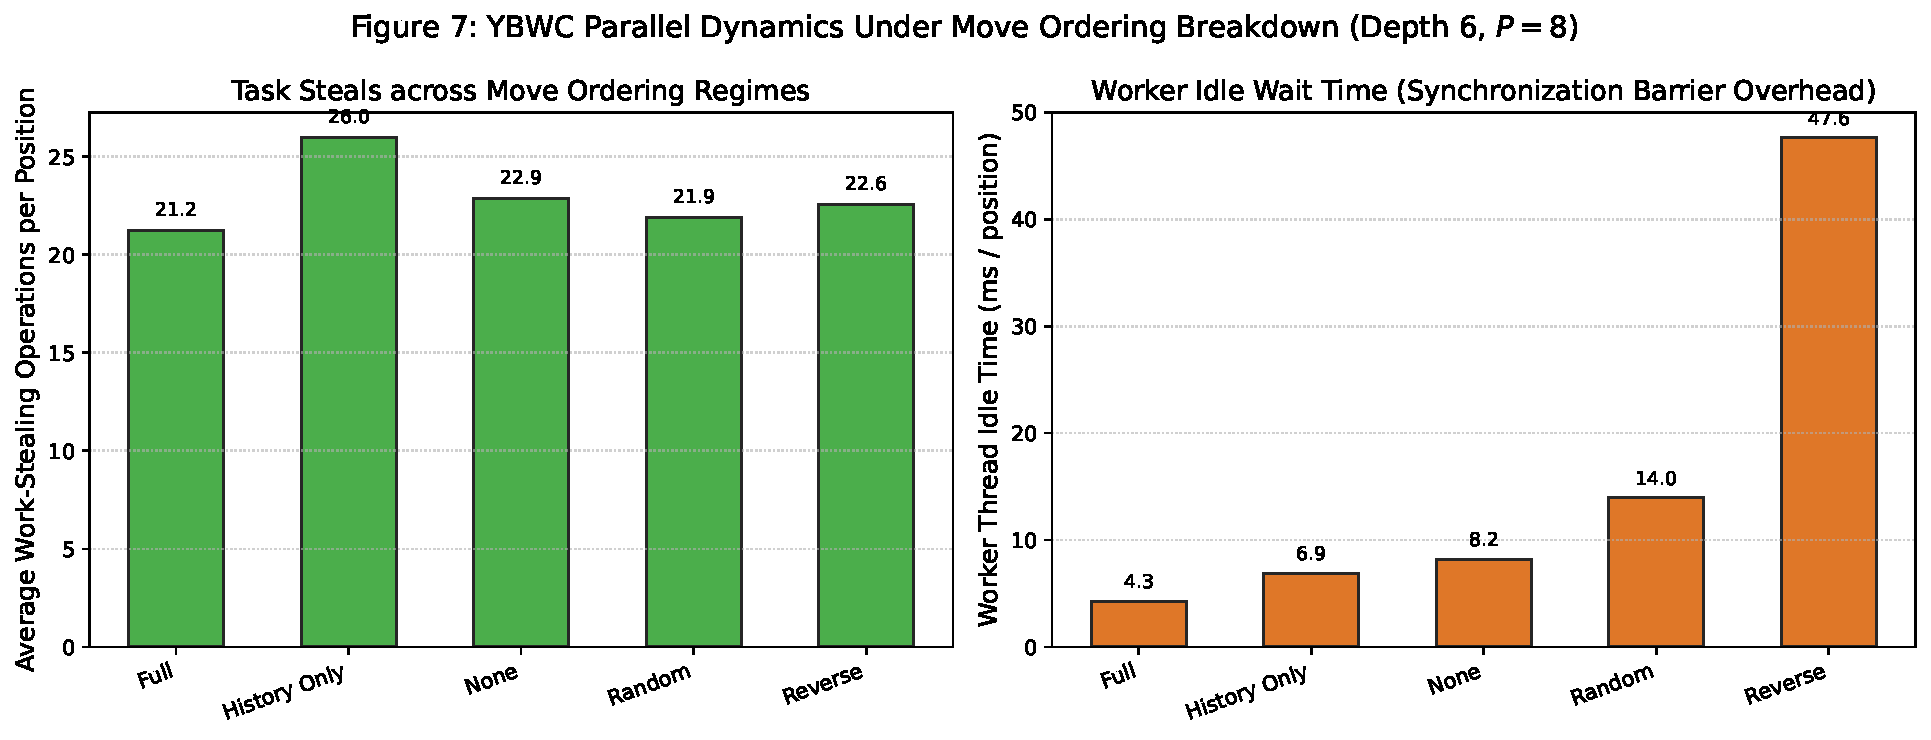
\includegraphics[width=0.95\textwidth]{figures/fig7_ybwc_steals_idle.pdf}
    \caption{YBWC Dynamics: Task Steals and Worker Synchronization Idle Time (Depth 6, $P=8$).}
    \label{fig:ybwc_dynamics}
\end{figure}

\subsection{Key Findings from Failure Analysis}
\begin{enumerate}
    \item \textbf{Asymptotic Tree Explosion:} In sequential search ($B_2$), moving from \texttt{full} to \texttt{reverse} ordering causes nodes to explode by \textbf{$86.8\times$} (from $5,486$ to $476,150$) and runtime to increase by \textbf{$61.6\times$}, empirically validating Knuth and Moore's worst-case theorem $\mathcal{O}(b^d)$.
    \item \textbf{Parallel Slowdown in Root Splitting ($P_1$):} Under \texttt{history\_only}, $P_1$ experiences a catastrophic search overhead explosion of \textbf{$+651.1\%$} ($76,925$ nodes vs $10,651$ for $B_2$). Consequently, 8-threaded $P_1$ runs in $4.94\text{ ms}$ while single-threaded $B_2$ runs in $3.28\text{ ms}$, producing a speedup of \textbf{$0.90\times$ (parallel slowdown)}.
    \item \textbf{PVS and YBWC Breakdown:} Under \texttt{history\_only}, search overhead exceeds $+100\%$ ($+115.4\%$ for PVS, $+101.3\%$ for YBWC) because the first move is frequently suboptimal, triggering expensive full-window re-searches in PVS and false ALL-node splits in YBWC.
    \item \textbf{Synchronization Idle Time Explosion:} As illustrated in Figure~\ref{fig:ybwc_dynamics}, worker thread idle wait time per position increases from $4.3\text{ ms}$ under \texttt{full} ordering to \textbf{$47.6\text{ ms}$} under \texttt{reverse} ordering (an $11\times$ surge). Asymmetric branch depths leave 7 threads idle while a single worker traverses an unpruned subtree.
\end{enumerate}

% ----------------------------------------------------
\section{Tournament Evaluation and GUI Interface}
\label{sec:tournament_gui}

\subsection{Head-to-Head Engine Tournament}
To evaluate practical playing strength, we conducted a round-robin tournament comprising 24 games with alternating colors and randomized 4-ply openings between: $B_0$ (Random), $B_0$ (Greedy), $B_2$ (Alpha-Beta, depth 6), and $P_3$ (YBWC, depth 6, $P=8$). 

As shown in Table~\ref{tab:tournament}, $P_3$ and $B_2$ achieved joint dominance with an \textbf{$83.3\%$ win rate} and an average disc margin of $+25.67$ and $+34.42$ discs over naive players. Greedy play ($B_0$) collapsed against deep heuristic lookahead ($33.3\%$ win rate), confirming that immediate disc maximization in Othello is strategically disastrous compared to mobility and corner-anchored evaluation.

\begin{table}[htbp]
  \centering
  \caption{Engine Tournament Standings (24 Matches, 4-Ply Random Opening Book)}
  \label{tab:tournament}
  \begin{tabular}{l c c c c c c c}
    \toprule
    \textbf{Contestant} & \textbf{Games} & \textbf{Wins} & \textbf{Draws} & \textbf{Losses} & \textbf{Win Rate} & \textbf{Mean Margin} & \textbf{95\% Conf. Interval} \\
    \midrule
    \textbf{YBWC ($P_3$, $P=8$)} & 12 & 10 & 0 & 2 & 83.3\% & +25.67 & $[+9.24, +42.10]$ \\
    \textbf{Seq $\alpha\beta$ ($B_2$)} & 12 & 10 & 0 & 2 & 83.3\% & +34.42 & $[+19.71, +49.13]$ \\
    \textbf{Greedy ($B_0$)}        & 12 & 4  & 0 & 8 & 33.3\% & -20.25 & $[-41.11, +0.61]$ \\
    \textbf{Random ($B_0$)}        & 12 & 0  & 0 & 12 & 0.0\%  & -39.83 & $[-48.75, -30.92]$ \\
    \bottomrule
  \end{tabular}
\end{table}

\subsection{Interactive Graphical Frontend}
A decoupled GUI was built using Pygame (\texttt{gui/app.py}), communicating via the engine's line-based CLI protocol. The interface renders an authentic green felt board, highlights legal moves, and provides an interactive side panel with algorithm/core selectors, search depth sliders, and a real-time telemetry dashboard. A dedicated \textit{Step-by-Step Analysis Mode} visualizes the candidate move computed by the engine before committing it to the board.

% ----------------------------------------------------
\section{Conclusion and Future Work}
\label{sec:conclusion}

This paper presented an empirical and theoretical comparative study of parallel alpha-beta search algorithms in Othello. By enforcing an identical bitboard engine, evaluation heuristic, and move ordering across all implementations, we isolated the pure algorithmic properties of Root Splitting ($P_1$), PVS ($P_2$), and YBWC ($P_3$). 

Our findings demonstrate that the Young Brothers Wait Concept achieves the best parallel efficiency ($95.8\%$ at $P=2$) by dynamically suppressing parallel branching at CUT-nodes. Conversely, naive Root Splitting is severely limited by branch load imbalance and collapses to parallel slowdown ($S_8 = 0.90\times$) under weak move ordering. Our failure analysis empirically verifies that parallel alpha-beta efficiency is fundamentally bound to sequential move-ordering quality.

\textbf{Future Work:} Promising research directions include: (1) integrating lock-free shared transposition tables across parallel threads to share bounds across distant tree branches, (2) extending YBWC to massively parallel GPU architectures~\cite{cohen2022high}, and (3) hybridizing parallel alpha-beta with Monte Carlo Tree Search~\cite{cazenave2021parallel}.

% --- References ---
\bibliographystyle{plain}
\bibliography{references}

\end{document}
